\section{Assuring Safe Perception}\label{sec:proofrule}
%Willem and Martin\\
%4,5 pages	concluded at page 13\\
\subsection{Classifier Analysis}
An ontology $\mathcal O=(\mathcal L,\sqcap,\sqcup)$ is a complete distributive lattice over a set $\mathcal L$ of labels. The unique complement of $l\in\mathcal L$ is denoted by $\overline l$. The induced non-strict partial order of $\mathcal O$ is denoted by $\sqsubseteq$ and its strict variant by $\sqsubset$. We say that a label $l\in\mathcal L$ is more specific (broader) than a label $l'\in\mathcal L$ if $l\sqsubset l'$ ($l'\sqsubset l$, respectively). A classifier $c_l$ for the label $l\in\mathcal L$ takes an artifact $a$ as input and returns a numerical value $c_l(a) \in [\min,\max]$ which corresponds to its degree of conviction that the artifact $a$ is of type $l$.
Given the upper threshold $g_l^+$ and the lower threshold $g_l^-$ with $g_l^+\geq g_l^-$ we define the label assignment for an artifact $a$ as follows
\begin{gather*}
    \Label(c_l,g_l^+,g_l^-)(a) = \left\{
    \begin{array}{ll}
    l & \text{ if } c_l(a) \geq g_l^+\\
    \overline l & \text{ if } c_l(a) < g_l^-\\
    \top & \text{ otherwise.}
    \end{array}\right.
\end{gather*}
We use the short notation $\Label(c_l)(a)$ when the thresholds are fixed. 

There are various quality measures for classifiers. A classifier is evaluated against a given a test data set $T$, where $T$ is a set of correct and complete labeled and representative set of artifacts. Hence, for each label $l\in\mathcal L$, we obtain a partitioning of $T=T(l) \cup T(\overline l)$ into the set $T(l)$ of artifacts which are labeled with $l$ and its complement $T(\overline l)$. The number of elements is denoted by $n_l$ and $n_{\overline l}$, respectively.

To analyze a classifier $c_l$ we are mainly interested in the relation between the threshold $g_l^+$, the true positive rate (\TPR), and the false positive rate (\FPR) on the one hand, and the relation between the threshold $g_l^-$, 
the true negative rate (\TNR), and the false negative rate (\FNR) on the other.
For each classifier we obtain two ROC curves (receiver operating characteristics):
\begin{itemize}
\item ROC curve $RP$ represents the relationship of $\TPR(g_l^+)$ and $\FPR(g_l^+)$,
where
\begin{gather*}
    \TPR(g_l^+) = \frac{ | T(l) \cap \{ c_l(a) \geq g_l^+ \}|}{|T(l)|},\quad
    \FPR(g_l^+) = \frac{ | T(\overline l) \cap \{ c_l(a) \geq g_l^+ \}|}{|T(\overline l)|}
\end{gather*}
\item ROC curve $RN$ represents the relationship of $\TNR(g_l^-)$ and $\FNR(g_l^-)$, where
\begin{gather*}
    \TNR(g_l^-) = \frac{ | T(\overline a) \cap \{c_l(a) < g_l^- \}|}{|T(\overline l)|},\quad
    \FNR(g_l^-) = \frac{ | T(l) \cap \{c_l(a) < g_l^- \}|}{|T(l)|}.
\end{gather*}
\end{itemize}
The rates as given above are measured against the fixed test data set.
According to Hoeffding's inequality we can derive the following bounds for the estimated false positive rates $\widehat\FPR$ and the estimated
false negative rate $\widehat\FNR$:
\begin{gather*}
    \FPR(g_l^+) + \epsilon \geq \widehat\FPR(g_l^+) \text{ with confidence $\beta$ if } \beta \leq 1 - e^{-2|T(\overline l)|\epsilon^2}\\
    \FNR(g_l^-) + \epsilon \geq \widehat\FNR(g_l^-) \text{ with confidence $\beta$ if } \beta \leq 1 - e^{-2|T(l)|\epsilon^2}
\end{gather*}
The situation is depicted in Fig. \ref{fig:ros}.
\begin{figure}
    \centering
    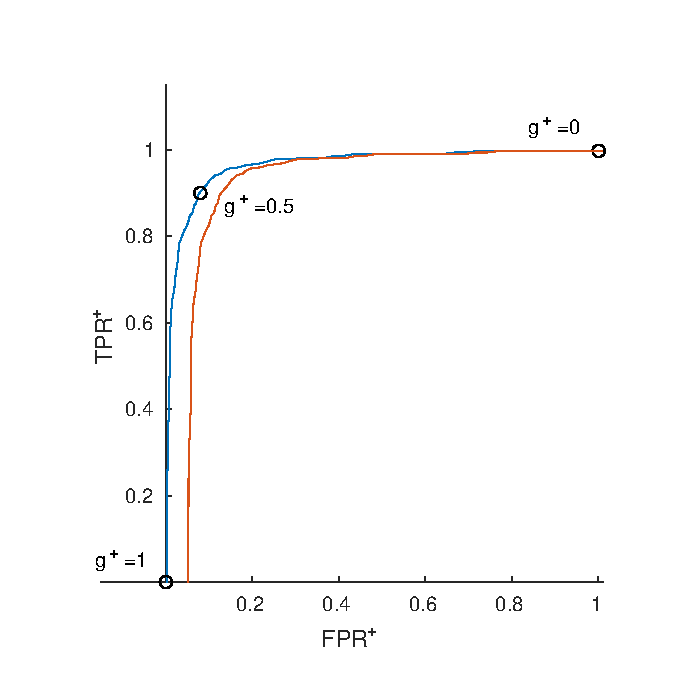
\includegraphics[width=0.5\textwidth]{ros}
    \caption{The ROS curve obtained by test data is depicted in blue, the $\epsilon$-margin for a $\beta$ confidence is shown in red.}
    \label{fig:ros}
\end{figure}

Note, that the rate above correspond to unknown conditional probabilities. E.g.\
$\widehat\FPR(g_l^+)$ represents the expected value of the conditional probability $p( c_l(a)\geq g_l^+ \mid a\in T(l))$.

\subsection{Classifier Optimization}
Let $\Phi$ be a formula that restricts the availability of a maneuver in favor of safety. 
E.g.\ $\Phi$ allows a fast transit of a critical passage only if it can be ensured that there a no humans on the sidewalk. In such a setting $\Phi = l_1 \land \l2 \land \dots \land l_n$ is a conjunction of literals $l_i=\lnot A_i$ of the form ``it is false that there is a human at cell $c_i$''. The truth value of each atom $A_i$ directly depends on a classifier output, which is, in our example, a human classifier. Our goal is to find an optimal threshold values for the related classifiers, separately for each cell,
such that the risk of missperception is restricted to a given safety bound
$\epsilon$ while the availability is maximized.

We want to ensure that the false positive rate of $\Phi$ is below a
given threshold $\epsilon$. Clearly, $\Phi$ is false if at least one literal
is a false positive. On the other hand, $\Phi$ is positive if and only if
all literals are positive. Taking both arguments together yields that
$\Phi$ is a false positive if and only if all literals are false positives.

Recall, that the false positive rates under consideration corresponds
to the expected value of conditional probabilities.
For stochastically independent events we have the identity 
$p(A_1|B_1)\cdot p(A_2|B_2) = p(A_1,A_2|B_1,B_2)$. Under the assumption that
the underlying classifiers of two literals are stochstically independent,
this allows us to represent the false negative rate of a conjunction as the
product of the literals. The same argument holds for the true positive rate.

Hence, we are allowed to distribute a given threshold $\epsilon$ for the
false positive rate of $\Phi$, i.e., $\FPR_\Phi+\epsilon\geq\widehat{\FPR_\Phi}$ to the literals $\prod\epsilon_i = \epsilon$ such that $\epsilon_i$
is an individual threshold for the false positive rate for the literals $l_i$.

%which -- in turn -- finally yields a threshold for the related classifiers, i.e., $\FPR(g^-)+\epsilon_i \geq  \widehat{\FPR(g^-)}$.
%
%Wie bekommen wir jetzt eine Abschätzung für die TP-Rate?
%Wir haben nun $g^-$ möglichst scharf gestellt.
%Wählen wir nun $g^- = g^+$, dann haben wir die Situation, dass wir größer oder gleich
%$g^-$ ist, suchen wir nun eine Einstellung für $g^+$, so dass wir, wenn



%We make the following assumption: 
%Let $c_l$ and $c_{l'}$ be two classifiers, where $l$ is more specific than $l'$. Then
%for quality measure and any thresholds for $c_l$ there exists thresholds for $c_{l'}$ 
%such that $c_{l'}$ is of equal of better quality than $c_l$.

%Before we proceed to give a precise definition of the label assignment of a fused classifier we introduce some additional concepts.
%\begin{itemize}
%\item A set of labels $L=\{l_1,\dots,l_n\}$ is consistent (with respect to the ontology)
%if $\bigsqcap\limits_{l\in L} l \neq \bot$. Otherwise, $L$ is called inconsistent (with %respect to the ontology).
%\item Let $L$ be inconsistent. A subset $L'\subseteq L$ is called a maximal consistent subset of $L$ if $L'$ is consistent and for any $l\in L\setminus L'$ the set $L'\cup\{l\}$ is inconsistent.
%\end{itemize}

We combine several classifiers $c_1,c_2,\dots, c_n$ with upper thresholds $g_1^+, g_2^+, \dots, g_n^+$ and lower thresholds $g_1^-, g_2^-, \dots, g_n^-$ using the vector notion $\mathbf c = (c_1,\dots,c_n)^T$, $\mathbf g^+=(g_1^+,\dots, g_n^+)^T$, $\mathbf g^-=(g_1^-,\dots,g_n^-)^T$. 

For any artifact $a$ we define the auxiliary sets
$P(a) = \{l_i\mid c_i(a) \geq g_i^+\}$ representing positive evidences and
$N(a) = \{\overline{l_i}\mid c_i(a) < g_i^-\}$ representing negative evidences.
The label assignment of the fused classifier is defined as follows
\begin{gather*}
    \mathrm{type}(a,\mathbf c, \mathbf g^+,\mathbf g^-) = 
    \underbrace{
    \bigsqcup\limits_{\substack{\text{$P$ is maximal}\\\text{consistent subset}\\\text{of $P(a)$}}} \bigsqcap\limits_{l \in P} l}_{\text{(A)}}
    \sqcap
    \underbrace{
    \bigsqcup\limits_{\substack{\text{$N$ is maximal}\\\text{consistent subset}\\\text{of $N(a)$}}} \bigsqcap\limits_{l \in N} l}_{\text{(B)}}
    %\bigsqcup\limits_{i\in P(a)} l_i \sqcap \bigsqcap\limits_{i\in N(a)} \overline{l_i},
\end{gather*}
with the convention that the expression $(A)$ evaluates to $\top$ if $P(a)$ is empty.
That is, positive and negative evidence are treated separately at first. 
Then consistent evidence is used to specialize the classification, whereas inconsistent evidence is used to broaden the classification.

\todo[inline]{WH: Ein etwas komplizierteres Beispiel: Wir haben positive Evidenzen Dackel, Katze und negative Evidenz fuer Hund. Die maximal konsistenten Mengen der positiven Evidenzen sind Dackel und Katze, wir bekommen also Tier. Zusammen mit der negativen Evidenz bekommen wir also, dass es sich um  ein Tier handelt, dass kein Hund ist. Macht das Sinn?
\\
Annaehrend. Tatsaechlich wird es sich wohl um eine Katze handeln. Begruendung. Jeder Testdatensatz fuer ein Dackel ist auch Testdatensatz fuer einen Hund. Es gibt mehr Testdatensaetze fuer den Hund. Nach Hoeffding muessen wir also mit mehr Unsicherheiten bei der Dackelklassifikation rechnen. Deshalb koennen wir also davon ausgehen, dass die Aussage kein Hund stimmt. Katze ist mit dieser Aussage konsistent.
\\
Ist dieses Argument valide? Was wir mit Sicherheit sagen koennen, ist dass die Erwartungswerte für den Hundeklassifikator sicherer als die Erwartungserte für den Dackel sind.}

\begin{example}
\begin{table}
$\begin{array}{cc|c}
    (1)&(2)&(3)\\
    \hline
    l_1 &l_2 & l_1 \sqcup l_2\\
    l_1 &\overline{l_2} & l_1\\
    l_1 &\top& l_1\\
    \overline{l_1} &l_2 & l_2\\
    \overline{l_1} &\overline{l_2} & \overline{l_1}\sqcap \overline{l_2}\\
    \overline{l_1} &\top& \overline{l_1}\\
    \top & l_2 & l_2\\
    \top & \overline{l_2} & \overline{l_2}\\
    \top & \top & \top
  \end{array}$
  \quad
  $\begin{array}{cc|c}
    (1)&(2)&(3)\\
    \hline
    l_1 &l_2 & l_1\\
    l_1 &\overline{l_2} & \bot\\
    l_1 &\top & l_1 \\
    \overline{l_1} &l_2 & l_2 \sqcap \overline{l_1}\\
    \overline{l_1} &\overline{l_2} & \overline{l_2}\\
    \overline{l_1} &\top & \overline{l_1}\\
    \top & l_2 & l_2\\
    \top &\overline{l_2} & \overline{l_2}\\
    \top & \top & \top
  \end{array}$
  \caption{ The left table shows the result of joining two classifiers with $l_1 \sqcap l_2=\bot$ and the right table shows the result of joining two classifiers with
  $l_1 \sqsubseteq l_2$.\\ Column (1) shows the result of $\mathrm{type}(a,c_1,g_1^+,g_1^⁻)$,
  column (2) the result of $\mathrm{type}(a,c_2,g_2^+,g_2^⁻)$, and
  column (3) the joined result of $\mathrm{type}(a,\mathbf c, \mathbf g^+, \mathbf g^⁻)$.}
\end{table}

\end{example}

\subsection{Classifier Optimization}
Let $\Phi$ be an Boolean combination of atoms $A_1$, \dots, $A_n$, where the truth value of the atoms depends on classifiers.
Assume $\Phi$ is a safety critical formula, i.e.\ whenever $\Phi$ holds, ego is only allowed to perform safe maneuvers. That is, we have to find optimal thresholds for the classifiers such that $\Phi$ becomes false only in sufficiently secured cases.

The truth value of $\Phi$ is given by the truth values of its atoms. In a first step, we analyze this dependency. A valuation $v$ of the atoms with uncertainties is a function that maps each atom to $0$, $1$ or $?$, where $0$ represents that the atom does not hold, $1$ represents that the atom holds, and $?$ represents that it is not known whether the atom holds or not. The resulting trivalent truth value for $\Phi$ can be computed by exploiting ontological dependencies between the atoms.\todo{Das habe ich zwar geschrieben, wie das im Detail aussieht, weiss ich ehrlich gesagt nicht.}. Since $\Phi$ is only allowed
to become false in sufficiently secured cases, we subsume the cases where 
$\Phi$ is unknown to the cases where $\Phi$ is true. The following table depicts all
valuations for the atoms under which $\Phi$ is true:
\begin{gather*}
  \begin{array}{ccccc|c}
    A_1& A_2 & A_3 & \dots & A_n & \Phi\\
    \hline
    1  &  ?  &    1 & \dots& 0   & 1\\
    1  &  1  &    1 & \dots& 0   & 1\\    
    1  &  ?  &    1 & \dots& 0   & 1\\    
    0  &  0  &    1 & \dots& 1   & 1\\
    \vdots & \vdots & \vdots & \vdots &\vdots & \vdots\\
    ?  &  ?  &    ? & \dots& ?   & 1
  \end{array}
\end{gather*}
There are some atoms $A_i$ for which either $v(A_i)=0$ or $v(A_i)=1$ can lead to a satisfying valuation for $\Phi$. These are exactly those atoms which occure with both polarities in a minimal conjunctive normal form of $\Phi$. For these atoms there is obviously no clear direction of optimization. Hence, we restrict our optimization to atoms occuring with one polarity in the minimal CNF. For simplicity, let us assume that the remaining atoms are of the form $A_i\equiv\textrm{label}(c_l,g_l^+,g_l^-)(a)=l$. Further assume, that $A_i$ occurs in positive polarity. 
That is, we want to assign thresholds $g_l^+$ and $g_l^-$ such that the classifier yields a false negative rate as small as possible while maintaining a sufficient high sensitivity.

\subsection{Adjusting Hoeffding's inequality}











